\hypertarget{group__tcp__raw}{}\section{T\+CP}
\label{group__tcp__raw}\index{T\+CP@{T\+CP}}
Collaboration diagram for T\+CP\+:
\nopagebreak
\begin{figure}[H]
\begin{center}
\leavevmode
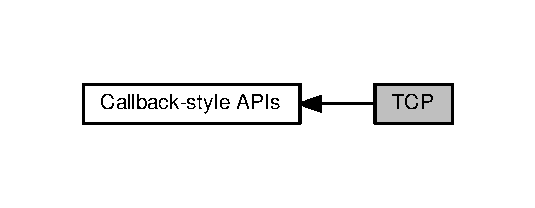
\includegraphics[width=257pt]{group__tcp__raw}
\end{center}
\end{figure}
Transmission Control Protocol for IP~\newline
\begin{DoxySeeAlso}{See also}
\hyperlink{raw_api}{lw\+IP A\+PI} and \hyperlink{group__netconn}{Netconn A\+PI}
\end{DoxySeeAlso}
Common functions for the T\+CP implementation, such as functinos for manipulating the data structures and the T\+CP timer functions. T\+CP functions related to input and output is found in tcp\+\_\+in.\+c and tcp\+\_\+out.\+c respectively.~\newline
